\section{Use case}
\subsection{System Actors}

{
\renewcommand{\arraystretch}{1.2}
\begin{longtable}{|>{\bfseries\raggedright\arraybackslash}p{0.2\textwidth}|>{\raggedright\arraybackslash}p{0.68\textwidth}|}
\caption{System actors}\label{tab:system-actors}\\
\hline
\textbf{Actor} & \textbf{Description} \\ \hline
\endfirsthead
\hline
\textbf{Actor} & \textbf{Description} \\ \hline
\endhead
User & Abstract actor representing any authenticated person using the system. It owns the common use cases Login, Logout, and Update Profile, which are inherited by all concrete human actors. \\ \hline
Student & Learner enrolled in one or more courses. Browses and registers for courses, accesses learning materials, takes quizzes, submits assignments, tracks progress, asks the AI assistant questions about course materials, and views personal learning risk warnings. \\ \hline
Teacher & Lecturer assigned to teach courses. Manages course materials, quizzes, and assignments, monitors enrolled students, and reviews at-risk students together with the explanations produced by the warning model. \\ \hline
Administrator & Staff member responsible for operating the system. Manages user accounts and roles, courses, classes and schedules, notifications, and system configuration. \\ \hline
AI Service & Supporting system actor that answers course-related questions using Retrieval-Augmented Generation and computes academic risk scores with their explanations. It is invoked by the backend and never acts on its own initiative. \\ \hline
\end{longtable}
}

\subsection{System use case diagram}

\subsubsection{System use case}

\begin{figure}[H]
    \centering
    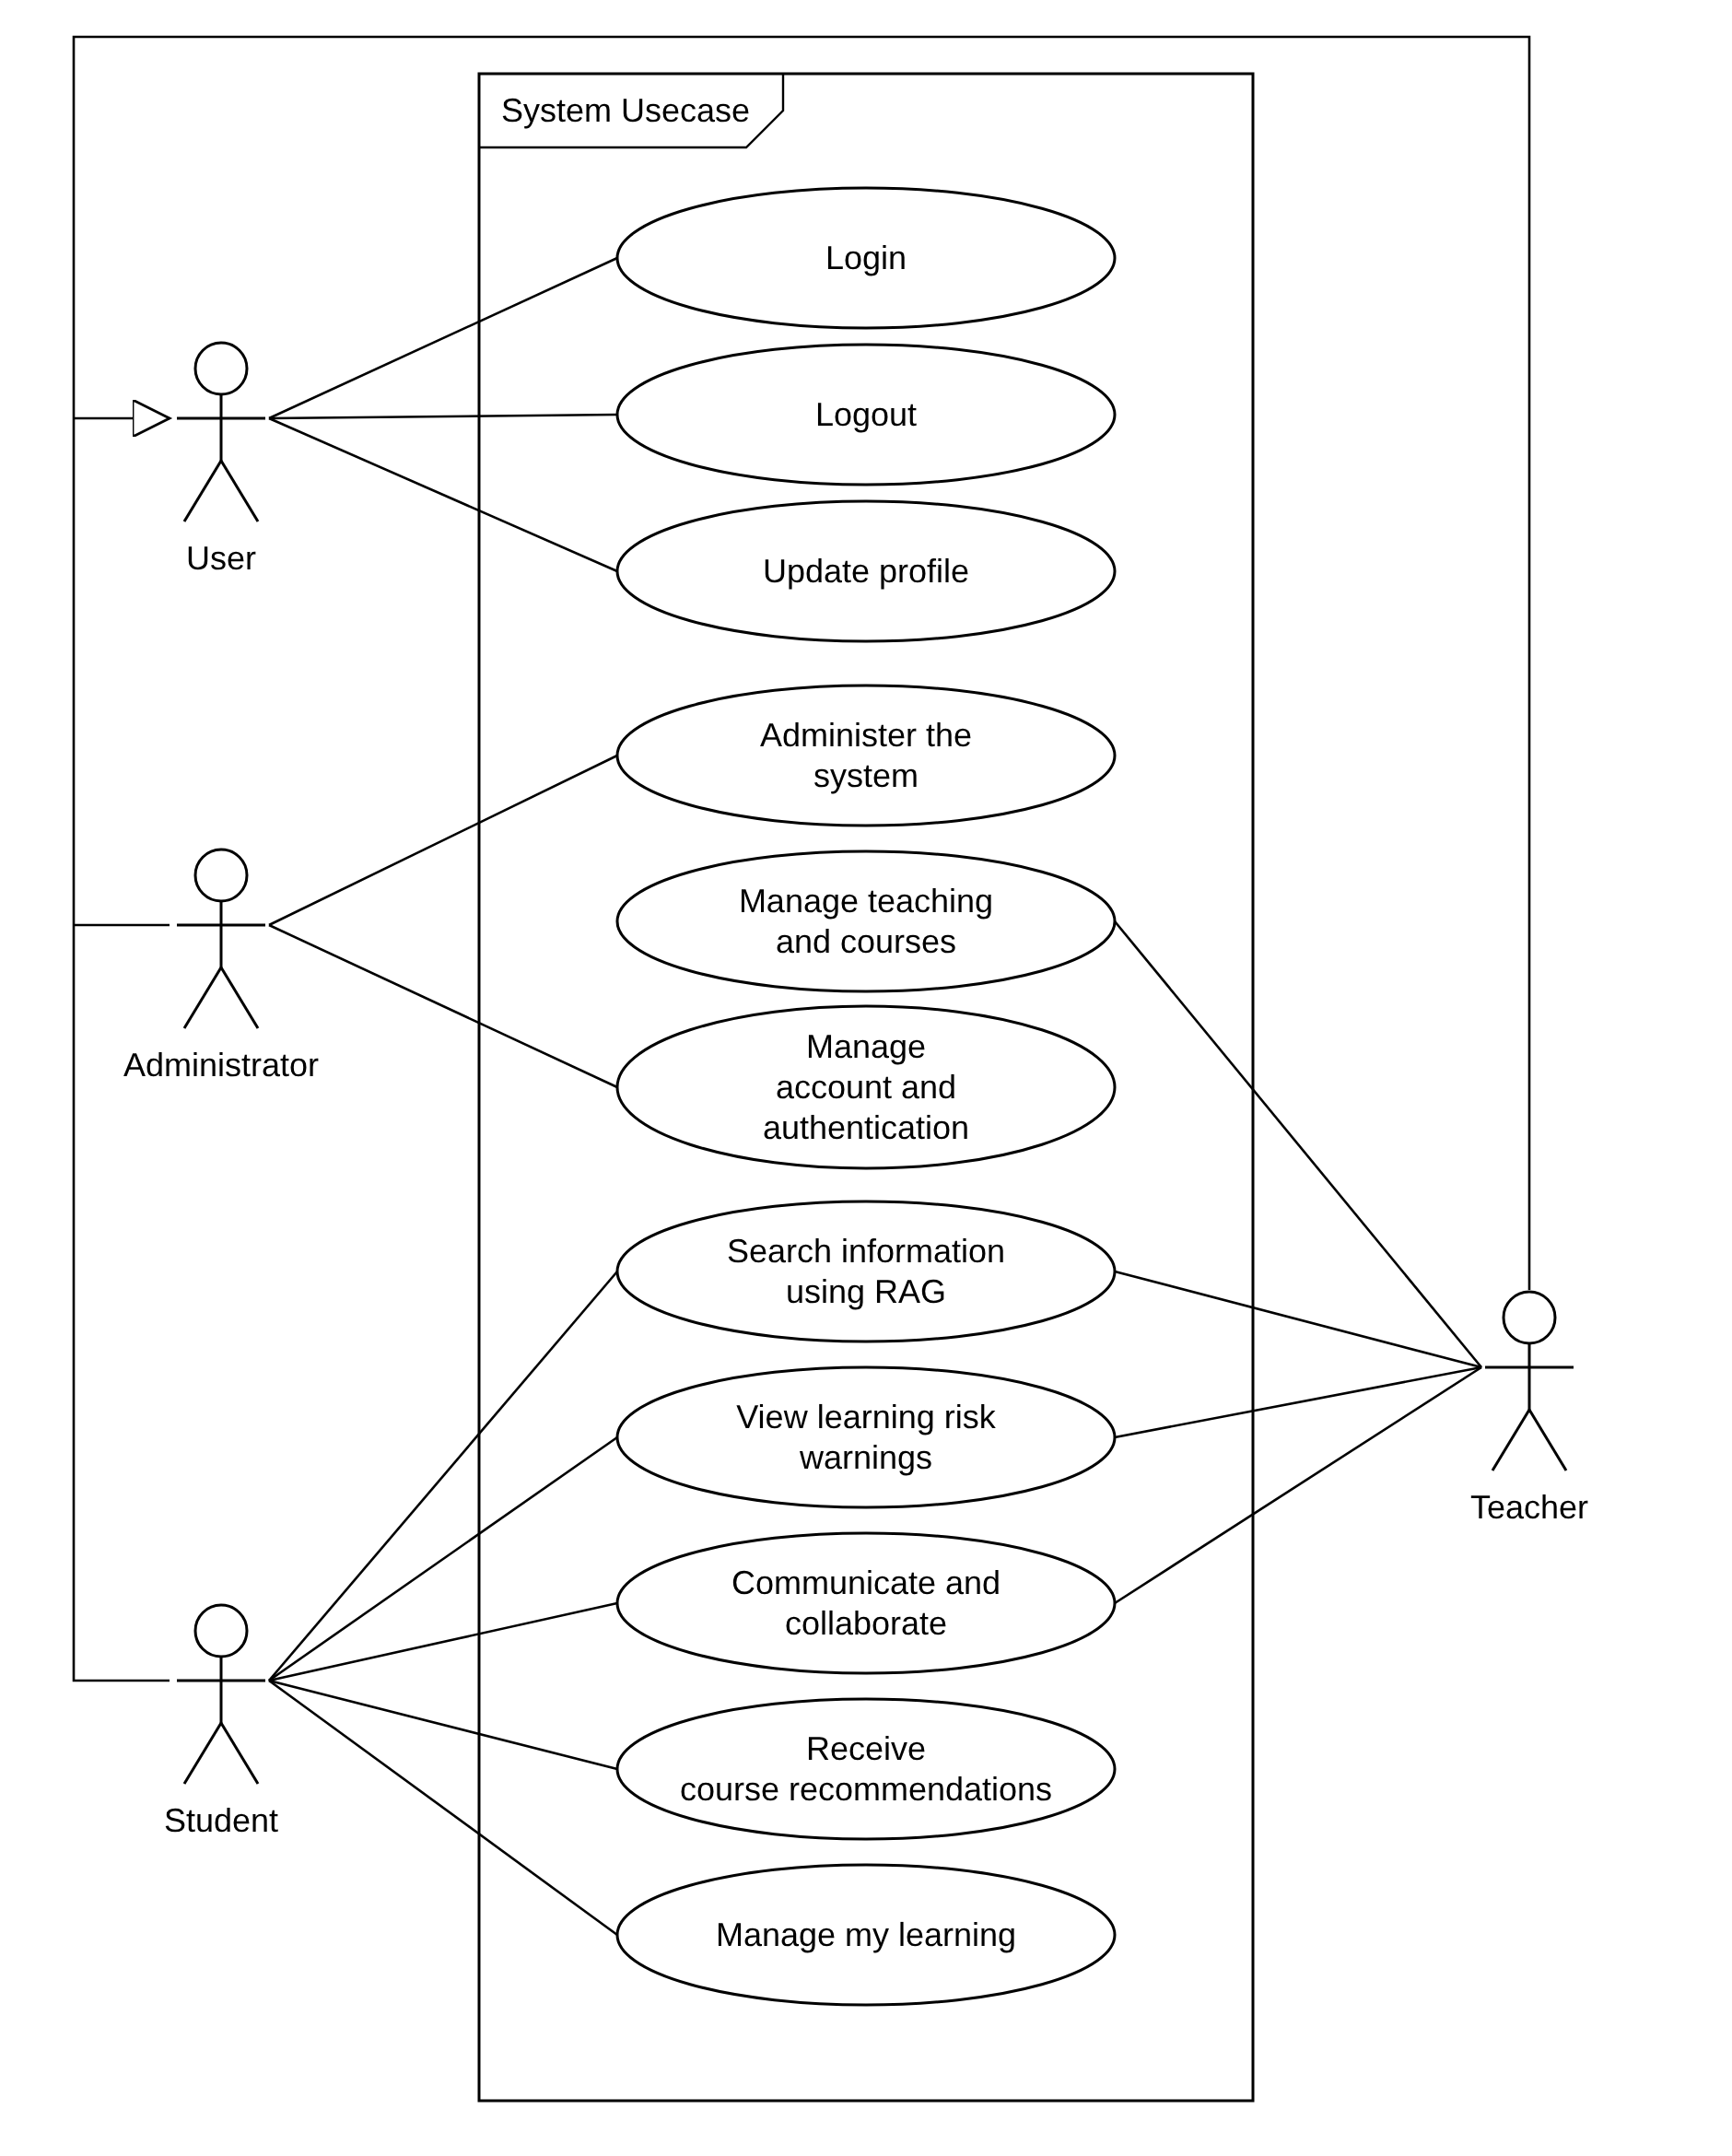
\includegraphics[width=0.7\textwidth, height=0.7\textheight, keepaspectratio]{images/usecase/system_usecase.png}
    \caption{System Use Case Diagram}
    \label{fig:system-usecase}
\end{figure}

{
\renewcommand{\arraystretch}{1.1}
\setlength{\tabcolsep}{8pt}
\begin{longtable}{|>{\bfseries\raggedright\arraybackslash}p{0.205\textwidth}|>{\raggedright\arraybackslash}p{0.685\textwidth}|}
\hline
Use-case ID & UC-USR-01 \\ \hline
Use-case name & Login \\ \hline
Author & Nguyen Manh Tri Minh \\ \hline
Description & Allows a user (Student, Teacher, or Administrator) to authenticate and access the features permitted by their role. \\ \hline
Actor & User (Student, Teacher, Administrator) \\ \hline
Trigger & The user opens the login page of the system portal. \\ \hline
Precondition &
1. The user has a valid, active account in the system. \par
2. The user is not currently logged in. \\ \hline
Postcondition & The user is authenticated, a secure session (access token) is issued, and the user can access system features according to their role. \\ \hline
Normal Flow &
1. The user enters their credentials (username or email and password). \par
2. The user submits the login form. \par
3. The system forwards the credentials to the authentication service and validates them against the user's account. \par
4. The system retrieves the user's role and permissions. \par
5. The system creates a secure session and issues an access token. \par
6. The system redirects the user to the dashboard corresponding to their role (student, teacher, or administrator dashboard). \\ \hline
Alternative Flow &
\textbf{A1: Valid session already exists} \par
1. At step 1, the system detects a valid, unexpired session for the user. \par
2. The system skips the login form and redirects the user directly to their dashboard. \\ \hline
Exception Flow &
\textbf{E1: Invalid credentials} \par
1. At step 3 of the normal flow, the credentials do not match any account. \par
2. The system rejects the login attempt, displays an error message, and prompts the user to try again. \par\vspace{4pt}
\textbf{E2: Account locked or suspended} \par
1. At step 3 of the normal flow, the system detects that the account is locked or suspended. \par
2. The system denies access and displays a message asking the user to contact the administrator. \par\vspace{4pt}
\textbf{E3: Authentication service unavailable} \par
1. At step 3 of the normal flow, the authentication service does not respond. \par
2. The system displays a temporary service error and allows the user to retry later. \\ \hline
\end{longtable}
}

{
\renewcommand{\arraystretch}{1.1}
\setlength{\tabcolsep}{8pt}
\begin{longtable}{|>{\bfseries\raggedright\arraybackslash}p{0.205\textwidth}|>{\raggedright\arraybackslash}p{0.685\textwidth}|}
\hline
Use-case ID & UC-USR-02 \\ \hline
Use-case name & Logout \\ \hline
Author & Nguyen Manh Tri Minh \\ \hline
Description & Allows a user to securely terminate their active session and leave the system. \\ \hline
Actor & User (Student, Teacher, Administrator) \\ \hline
Trigger & The user selects the logout function from the navigation menu. \\ \hline
Precondition & The user is currently logged into the system. \\ \hline
Postcondition & The user's session is terminated and the access token can no longer be used. \\ \hline
Normal Flow &
1. The user clicks the logout button. \par
2. The system invalidates the active session and clears the authentication tokens stored on the client. \par
3. The system redirects the user to the login page. \\ \hline
Alternative Flow &
\textbf{A1: Automatic logout after inactivity} \par
1. The user remains inactive for longer than the configured session timeout. \par
2. The system invalidates the session automatically. \par
3. On the next request, the system redirects the user to the login page. \\ \hline
Exception Flow &
\textbf{E1: Session already expired} \par
1. At step 2 of the normal flow, the system detects that the session has already expired. \par
2. The system redirects the user to the login page without displaying an error. \\ \hline
\end{longtable}
}

{
\renewcommand{\arraystretch}{1.1}
\setlength{\tabcolsep}{8pt}
\begin{longtable}{|>{\bfseries\raggedright\arraybackslash}p{0.205\textwidth}|>{\raggedright\arraybackslash}p{0.685\textwidth}|}
\hline
Use-case ID & UC-USR-03 \\ \hline
Use-case name & Update Profile \\ \hline
Author & Nguyen Manh Tri Minh \\ \hline
Description & Allows a user to view and update the editable fields of their personal profile, such as phone number, avatar, and personal email. Identity fields managed by the university (user ID, full name, role) are read-only. \\ \hline
Actor & User (Student, Teacher, Administrator) \\ \hline
Trigger & The user selects the option to view or edit their personal profile. \\ \hline
Precondition & The user is authenticated and logged into the system. \\ \hline
Postcondition & The updated profile information is saved and reflected throughout the system. \\ \hline
Normal Flow &
1. The user opens the profile page. \par
2. The system displays the current profile information, with editable fields enabled and identity fields shown as read-only. \par
3. The user updates the editable fields (e.g., phone number, avatar, personal email). \par
4. The user submits the form. \par
5. The system validates the data formats and checks that no read-only field has been changed. \par
6. The system saves the updated information. \par
7. The system confirms that the profile has been updated successfully. \\ \hline
Alternative Flow &
\textbf{A1: Cancel editing} \par
1. At step 3 or 4, the user selects ``Cancel''. \par
2. The system discards the changes and displays the unchanged profile. \\ \hline
Exception Flow &
\textbf{E1: Invalid data format} \par
1. At step 5 of the normal flow, a field contains malformed data (e.g., an invalid email address or an unsupported image format). \par
2. The system highlights the invalid field and requests correction; the profile is not updated. \par\vspace{4pt}
\textbf{E2: Save failure} \par
1. At step 6 of the normal flow, the system fails to save the changes. \par
2. The system displays an error message and keeps the previous profile information. \\ \hline
\end{longtable}
}


\subsubsection{Student use case}

\begin{figure}[H]
    \centering
    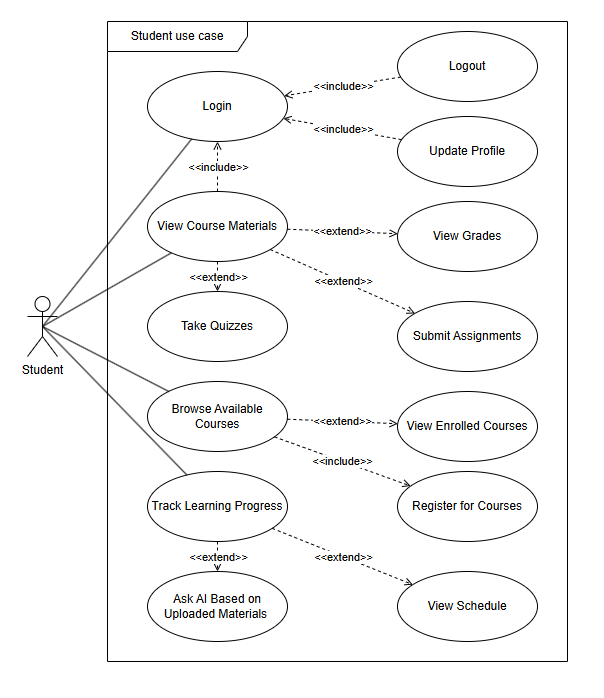
\includegraphics[width=0.5\textwidth, height=0.5\textheight, keepaspectratio]{images/usecase/student-usecase.png}
    \caption{Student Use Case Diagram}
    \label{fig:student-usecase}
\end{figure}


{
\renewcommand{\arraystretch}{1.1}
\setlength{\tabcolsep}{8pt}
\begin{longtable}{|>{\bfseries\raggedright\arraybackslash}p{0.205\textwidth}|>{\raggedright\arraybackslash}p{0.70\textwidth}|}
\hline
Use-case ID & UC-STU-01 \\ \hline
Use-case name & Login \\ \hline
Author & Dinh Cao Thien Loc \\ \hline
Description & Allows the student to authenticate and log into the system to access their personal dashboard and academic features. \\ \hline
Actor & Student \\ \hline
Trigger & The Student accesses the system's login portal. \\ \hline
Precondition &
1. The Student has a valid, active account in the system. \par
2. The Student is not currently logged in. \\ \hline
Postcondition & The Student is authenticated and can access system features according to their role. \\ \hline
Normal Flow &
1. The Student enters their credentials (e.g., username/email and password). \par
2. The Student submits the login form. \par
3. The system validates the entered credentials against the database. \par
4. If validation succeeds, the system authenticates the Student and generates a secure session. \par
5. The system redirects the Student to the student dashboard. \\ \hline
Alternative Flow & N/A. \\ \hline
Exception Flow &
\textbf{E1: Invalid credentials} \par
1. At step 3 of the normal flow, the credentials do not match the database. \par
2. The system rejects the login attempt, displays an error message, and prompts the Student to try again. \par\vspace{4pt}
\textbf{E2: Account locked or suspended} \par
1. At step 3 of the normal flow, the system detects the account is locked. \par
2. The system denies access and displays a contact support message. \\ \hline
\end{longtable}
}

{
\renewcommand{\arraystretch}{1.1}
\setlength{\tabcolsep}{8pt}
\begin{longtable}{|>{\bfseries\raggedright\arraybackslash}p{0.205\textwidth}|>{\raggedright\arraybackslash}p{0.70\textwidth}|}
\hline
Use-case ID & UC-STU-02 \\ \hline
Use-case name & Logout \\ \hline
Author & Dinh Cao Thien Loc \\ \hline
Description & Allows the student to securely terminate their active session and leave the system. \\ \hline
Actor & Student \\ \hline
Trigger & The Student selects the logout function from the navigation menu. \\ \hline
Precondition & The Student is currently logged into the system. \\ \hline
Postcondition & The Student's session is completely terminated. \\ \hline
Normal Flow &
1. The Student clicks the logout button. \par
2. The system terminates the active user session and clears authentication tokens. \par
3. The system redirects the Student to the login page or public homepage. \\ \hline
Alternative Flow & N/A. \\ \hline
Exception Flow &
\textbf{E1: Session already expired} \par
1. At step 2 of the normal flow, the system detects the session has already expired. \par
2. The system safely redirects the Student to the login page without error. \\ \hline
\end{longtable}
}

{
\renewcommand{\arraystretch}{1.1}
\setlength{\tabcolsep}{8pt}
\begin{longtable}{|>{\bfseries\raggedright\arraybackslash}p{0.205\textwidth}|>{\raggedright\arraybackslash}p{0.70\textwidth}|}
\hline
Use-case ID & UC-STU-03 \\ \hline
Use-case name & Update Profile \\ \hline
Author & Dinh Cao Thien Loc \\ \hline
Description & Allows the student to modify and update allowable personal information such as phone number, avatar, and personal email. \\ \hline
Actor & Student \\ \hline
Trigger & The Student selects the option to edit their personal profile. \\ \hline
Precondition & The Student is authenticated and logged into the system. \\ \hline
Postcondition & The Student's updated profile information is saved and reflected in the system. \\ \hline
Normal Flow &
1. The Student opens the profile management section. \par
2. The system displays the current profile information in an editable form. \par
3. The Student updates allowable fields (e.g., phone number, avatar, personal email). \par
4. The Student submits the updated form. \par
5. The system validates the data formats and checks for any prohibited changes. \par
6. The system saves the updated information to the database. \par
7. The system confirms that the profile has been updated successfully. \\ \hline
Alternative Flow & N/A. \\ \hline
Exception Flow &
\textbf{E1: Invalid data format} \par
1. At step 5 of the normal flow, the user inputs malformed data (e.g., malformed email). \par
2. The system identifies the problem, highlights the field, and requests correction; the profile is not updated. \\ \hline
\end{longtable}
}

{
\renewcommand{\arraystretch}{1.1}
\setlength{\tabcolsep}{8pt}
\begin{longtable}{|>{\bfseries\raggedright\arraybackslash}p{0.205\textwidth}|>{\raggedright\arraybackslash}p{0.70\textwidth}|}
\hline
Use-case ID & UC-STU-04 \\ \hline
Use-case name & Browse Available Courses \\ \hline
Author & Dinh Cao Thien Loc \\ \hline
Description & Allows the student to view, search, and filter the catalog of available courses for the upcoming or current semester. \\ \hline
Actor & Student \\ \hline
Trigger & The Student navigates to the course catalog or registration section. \\ \hline
Precondition &
1. The Student is authenticated. \par
2. The system has active courses configured for the upcoming or current semester. \\ \hline
Postcondition & The Student successfully views the available courses and their details. \\ \hline
Normal Flow &
1. The Student opens the course catalog interface. \par
2. The system retrieves the list of available courses and displays them. \par
3. The Student uses search filters (e.g., department, schedule, lecturer) to find specific courses. \par
4. The system updates the displayed list based on the selected filters. \par
5. The Student clicks on a specific course to view detailed information (description, credits, prerequisites). \\ \hline
Alternative Flow & N/A. \\ \hline
Exception Flow &
\textbf{E1: No courses match the search filters} \par
1. At step 4 of the normal flow, no courses match the applied filters. \par
2. The system displays a ``No courses found'' message. \\ \hline
\end{longtable}
}

{
\renewcommand{\arraystretch}{1.1}
\setlength{\tabcolsep}{8pt}
\begin{longtable}{|>{\bfseries\raggedright\arraybackslash}p{0.205\textwidth}|>{\raggedright\arraybackslash}p{0.70\textwidth}|}
\hline
Use-case ID & UC-STU-05 \\ \hline
Use-case name & Register for Courses \\ \hline
Author & Dinh Cao Thien Loc \\ \hline
Description & Allows the student to officially enroll in a specific course or section during the registration period. \\ \hline
Actor & Student \\ \hline
Trigger & The Student selects the function to register for a specific course/section. \\ \hline
Precondition &
1. The Student is authenticated. \par
2. The course registration period is officially open. \\ \hline
Postcondition & The Student is officially enrolled in the course, and the available seat count is decreased by one. \\ \hline
Normal Flow &
1. The Student views an available course and clicks the ``Register'' button. \par
2. The system checks the Student's eligibility (e.g., prerequisites passed, maximum credit limit not exceeded, schedule conflicts). \par
3. The system checks if there are available seats in the selected course section. \par
4. The system records the Student's enrollment in the course. \par
5. The system confirms the successful registration. \\ \hline
Alternative Flow & N/A. \\ \hline
Exception Flow &
\textbf{E1: Prerequisites not met} \par
1. At step 2 of the normal flow, the student does not meet the course prerequisites. \par
2. The system denies registration and lists the missing prerequisite courses. \par\vspace{4pt}
\textbf{E2: Class is full} \par
1. At step 3 of the normal flow, there are no available seats. \par
2. The system denies registration and offers an option to join a waitlist (if applicable). \par\vspace{4pt}
\textbf{E3: Schedule conflict} \par
1. At step 2 of the normal flow, the system detects a scheduling conflict with existing enrollments. \par
2. The system highlights the overlapping courses and denies registration. \\ \hline
\end{longtable}
}

{
\renewcommand{\arraystretch}{1.1}
\setlength{\tabcolsep}{8pt}
\begin{longtable}{|>{\bfseries\raggedright\arraybackslash}p{0.205\textwidth}|>{\raggedright\arraybackslash}p{0.70\textwidth}|}
\hline
Use-case ID & UC-STU-06 \\ \hline
Use-case name & View Enrolled Courses \\ \hline
Author & Dinh Cao Thien Loc \\ \hline
Description & Allows the student to view a list of all courses they are currently enrolled in via their dashboard. \\ \hline
Actor & Student \\ \hline
Trigger & The Student navigates to their personal dashboard or ``My Courses'' section. \\ \hline
Precondition & The Student is authenticated. \\ \hline
Postcondition & The Student views their current enrollments. \\ \hline
Normal Flow &
1. The Student selects the ``My Courses'' tab. \par
2. The system queries the database for all active enrollments linked to the Student. \par
3. The system displays a list of the enrolled courses, including basic details (course name, lecturer, quick links to materials). \\ \hline
Alternative Flow & N/A. \\ \hline
Exception Flow &
\textbf{E1: No enrolled courses} \par
1. At step 2 of the normal flow, the student has no active enrollments. \par
2. The system displays an empty state message encouraging them to register. \\ \hline
\end{longtable}
}

{
\renewcommand{\arraystretch}{1.1}
\setlength{\tabcolsep}{8pt}
\begin{longtable}{|>{\bfseries\raggedright\arraybackslash}p{0.205\textwidth}|>{\raggedright\arraybackslash}p{0.70\textwidth}|}
\hline
Use-case ID & UC-STU-07 \\ \hline
Use-case name & View Course Materials \\ \hline
Author & Dinh Cao Thien Loc \\ \hline
Description & Allows the student to access, view, or download learning materials uploaded by the lecturer for a specific course. \\ \hline
Actor & Student \\ \hline
Trigger & The Student selects a specific course and navigates to the ``Materials'' or ``Modules'' section. \\ \hline
Precondition &
1. The Student is authenticated and officially enrolled in the requested course. \par
2. The Lecturer has uploaded materials to the course. \\ \hline
Postcondition & The Student successfully accesses the learning material. \\ \hline
Normal Flow &
1. The Student clicks on a document, video, or link provided in the course syllabus. \par
2. The system verifies the Student's access permissions for that specific material. \par
3. The system displays or downloads the requested material to the Student's device. \\ \hline
Alternative Flow & N/A. \\ \hline
Exception Flow &
\textbf{E1: Material is locked or not yet published} \par
1. At step 2 of the normal flow, the material is restricted by date or condition. \par
2. The system denies access and shows the date/condition when it will be available. \\ \hline
\end{longtable}
}

{
\renewcommand{\arraystretch}{1.1}
\setlength{\tabcolsep}{8pt}
\begin{longtable}{|>{\bfseries\raggedright\arraybackslash}p{0.205\textwidth}|>{\raggedright\arraybackslash}p{0.70\textwidth}|}
\hline
Use-case ID & UC-STU-08 \\ \hline
Use-case name & View Grades \\ \hline
Author & Dinh Cao Thien Loc \\ \hline
Description & Allows the student to view their assessment scores, cumulative GPA, and feedback provided by the lecturer. \\ \hline
Actor & Student \\ \hline
Trigger & The Student navigates to the ``Grades'' or ``Academic Record'' section. \\ \hline
Precondition &
1. The Student is authenticated and enrolled in courses. \par
2. Grades have been published by the Lecturer or system. \\ \hline
Postcondition & The Student successfully views their academic performance. \\ \hline
Normal Flow &
1. The Student selects a specific course to view detailed grades or views the cumulative GPA dashboard. \par
2. The system retrieves the published assessment scores (quizzes, assignments, midterms, finals) for that Student. \par
3. The system displays the grades, weightages, and any feedback provided by the Lecturer. \\ \hline
Alternative Flow & N/A. \\ \hline
Exception Flow &
\textbf{E1: Grades are hidden or not yet published} \par
1. At step 2 of the normal flow, the requested grades are not yet published. \par
2. The system displays a ``Pending'' or ``Not Available'' status for those specific assessments. \\ \hline
\end{longtable}
}

{
\renewcommand{\arraystretch}{1.1}
\setlength{\tabcolsep}{8pt}
\begin{longtable}{|>{\bfseries\raggedright\arraybackslash}p{0.205\textwidth}|>{\raggedright\arraybackslash}p{0.70\textwidth}|}
\hline
Use-case ID & UC-STU-09 \\ \hline
Use-case name & Take Quizzes \\ \hline
Author & Dinh Cao Thien Loc \\ \hline
Description & Allows the student to attempt and submit an active online quiz within a scheduled time frame. \\ \hline
Actor & Student \\ \hline
Trigger & The Student selects an active quiz to begin an attempt. \\ \hline
Precondition &
1. The Student is authenticated and enrolled in the course. \par
2. An active quiz is available and open for submission within the scheduled time frame. \\ \hline
Postcondition & The quiz attempt is saved, timestamped, and queued for grading (or auto-graded). \\ \hline
Normal Flow &
1. The Student clicks ``Start Quiz''. \par
2. The system records the start time and displays the quiz questions. \par
3. The Student selects/enters answers for the questions. \par
4. The Student clicks ``Submit Quiz''. \par
5. The system saves the answers, records the submission time, and closes the attempt. \par
6. The system auto-grades the objective questions (if configured) and provides a submission confirmation. \\ \hline
Alternative Flow & N/A. \\ \hline
Exception Flow &
\textbf{E1: Time expires before submission} \par
1. During step 3 of the normal flow, the allocated quiz time runs out. \par
2. The system automatically forces a submission of the currently saved answers. \par\vspace{4pt}
\textbf{E2: Attempt limit reached} \par
1. At step 1 of the normal flow, the system detects the student has used all allowed attempts. \par
2. The system prevents the Student from starting a new attempt. \\ \hline
\end{longtable}
}

{
\renewcommand{\arraystretch}{1.1}
\setlength{\tabcolsep}{8pt}
\begin{longtable}{|>{\bfseries\raggedright\arraybackslash}p{0.205\textwidth}|>{\raggedright\arraybackslash}p{0.70\textwidth}|}
\hline
Use-case ID & UC-STU-10 \\ \hline
Use-case name & Submit Assignments \\ \hline
Author & Dinh Cao Thien Loc \\ \hline
Description & Allows the student to upload file attachments or text submissions into an open assignment dropbox. \\ \hline
Actor & Student \\ \hline
Trigger & The Student navigates to an assignment and chooses to upload their work. \\ \hline
Precondition &
1. The Student is authenticated and enrolled in the course. \par
2. An assignment dropbox is open and accepting submissions. \\ \hline
Postcondition & The assignment file is securely stored and available for the Lecturer to grade. \\ \hline
Normal Flow &
1. The Student clicks ``Submit Assignment''. \par
2. The system displays the file upload or text entry interface. \par
3. The Student uploads the required files or enters text. \par
4. The Student confirms and submits. \par
5. The system verifies file types and size limits. \par
6. The system saves the submission, timestamps it, and links it to the Student and assignment. \par
7. The system displays a success receipt. \\ \hline
Alternative Flow & N/A. \\ \hline
Exception Flow &
\textbf{E1: Invalid file type or size exceeded} \par
1. At step 5 of the normal flow, the file does not meet constraints. \par
2. The system rejects the file and prompts the Student to upload a valid format. \par\vspace{4pt}
\textbf{E2: Past deadline} \par
1. At step 4 of the normal flow, the deadline has already passed. \par
2. The system either rejects the submission (if hard deadline) or marks it visually as ``Late'' (if soft deadline). \\ \hline
\end{longtable}
}

{
\renewcommand{\arraystretch}{1.1}
\setlength{\tabcolsep}{8pt}
\begin{longtable}{|>{\bfseries\raggedright\arraybackslash}p{0.205\textwidth}|>{\raggedright\arraybackslash}p{0.70\textwidth}|}
\hline
Use-case ID & UC-STU-11 \\ \hline
Use-case name & Track Learning Progress \\ \hline
Author & Dinh Cao Thien Loc \\ \hline
Description & Allows the student to monitor their completion percentage and remaining tasks for a specific course. \\ \hline
Actor & Student \\ \hline
Trigger & The Student views the course homepage or dashboard. \\ \hline
Precondition & The Student is authenticated and enrolled in courses that utilize progress tracking. \\ \hline
Postcondition & The Student views an accurate reflection of their course completion status. \\ \hline
Normal Flow &
1. The Student opens a specific course. \par
2. The system calculates the completion percentage based on viewed materials, completed quizzes, and submitted assignments. \par
3. The system displays a visual progress bar or checklist to the Student. \\ \hline
Alternative Flow & N/A. \\ \hline
Exception Flow &
\textbf{E1: Course does not utilize completion tracking} \par
1. At step 2 of the normal flow, progress tracking is disabled by the lecturer. \par
2. The system hides the progress bar interface. \\ \hline
\end{longtable}
}

{
\renewcommand{\arraystretch}{1.1}
\setlength{\tabcolsep}{8pt}
\begin{longtable}{|>{\bfseries\raggedright\arraybackslash}p{0.205\textwidth}|>{\raggedright\arraybackslash}p{0.70\textwidth}|}
\hline
Use-case ID & UC-STU-12 \\ \hline
Use-case name & View Schedule \\ \hline
Author & Dinh Cao Thien Loc \\ \hline
Description & Allows the student to view their academic timetable, including classes, assignment deadlines, and exam dates on a calendar interface. \\ \hline
Actor & Student \\ \hline
Trigger & The Student navigates to the ``Schedule'' or ``Calendar'' module. \\ \hline
Precondition &
1. The Student is authenticated and enrolled in at least one course. \par
2. Classes and events are mapped to a timetable. \\ \hline
Postcondition & The Student successfully views their academic timetable and upcoming deadlines. \\ \hline
Normal Flow &
1. The Student opens the calendar view (daily, weekly, or monthly). \par
2. The system retrieves class timings, assignment deadlines, and exam dates related to the Student's enrollments. \par
3. The system plots these events onto a visual calendar interface. \par
4. The Student clicks on a specific event to view location, time, and details. \\ \hline
Alternative Flow & N/A. \\ \hline
Exception Flow &
\textbf{E1: No scheduled events} \par
1. At step 2 of the normal flow, there are no events in the selected timeframe. \par
2. The system displays an empty calendar grid for the selected time period. \\ \hline
\end{longtable}
}

{
\renewcommand{\arraystretch}{1.1}
\setlength{\tabcolsep}{8pt}
\begin{longtable}{|>{\bfseries\raggedright\arraybackslash}p{0.205\textwidth}|>{\raggedright\arraybackslash}p{0.70\textwidth}|}
\hline
Use-case ID & UC-STU-13 \\ \hline
Use-case name & Ask AI Questions Based on Uploaded/Course Materials \\ \hline
Author & Dinh Cao Thien Loc \\ \hline
Description & Allows the student to ask questions and receive AI-generated answers grounded exclusively in the uploaded materials of the course. \\ \hline
Actor & Student \\ \hline
Trigger & The Student opens the AI learning assistant interface within a course and submits a question. \\ \hline
Precondition &
1. The Student is authenticated and enrolled in the course. \par
2. The AI module is active, and course materials have been successfully indexed into the system's vector database. \\ \hline
Postcondition & The Student receives a contextual, accurate answer based strictly on the course materials. \\ \hline
Normal Flow &
1. The Student types an academic question into the AI chat interface and presses send. \par
2. The system receives the query and retrieves relevant context exclusively from the specific course's uploaded materials (RAG approach). \par
3. The AI engine processes the question alongside the retrieved context to generate an accurate response. \par
4. The system displays the AI-generated answer to the Student, including citations/references to the specific uploaded course documents. \\ \hline
Alternative Flow & N/A. \\ \hline
Exception Flow &
\textbf{E1: Question is unrelated to course material} \par
1. At step 3 of the normal flow, the AI finds no relevant context in the course materials. \par
2. The AI responds that it cannot find the answer in the provided course context. \par\vspace{4pt}
\textbf{E2: AI service timeout/unavailability} \par
1. At step 2 or 3 of the normal flow, the AI service fails to respond in time. \par
2. The system displays a temporary error message advising the Student to try again later. \par\vspace{4pt}
\textbf{E3: Safety/Policy violation in prompt} \par
1. At step 2 of the normal flow, the student's prompt violates safety filters. \par
2. The system blocks the query and displays a warning regarding acceptable use. \\ \hline
\end{longtable}
}

\subsubsection{Admin use case}
\begin{figure}[H]
    \centering
    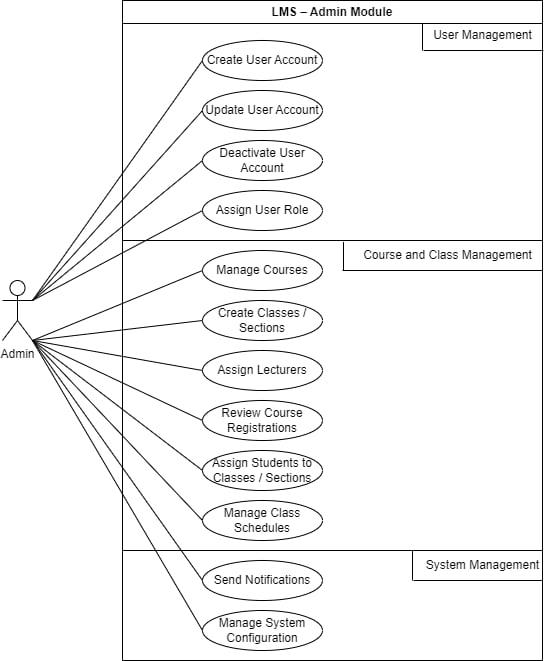
\includegraphics[width=0.8\textwidth, height=0.7\textheight, keepaspectratio]{images/usecase/AdminUsecase.png}
    \caption{Admin Use Case Diagram}
    \label{fig:admin-usecase}
\end{figure}


% ==========================================
% Admin Use Case Descriptions
% ==========================================

\renewcommand{\arraystretch}{1.1}
\setlength{\tabcolsep}{8pt}

% ==========================================
% UC-ADM-01: Create User Account
% ==========================================
\begin{longtable}{|>{\bfseries\raggedright\arraybackslash}p{0.205\textwidth}|>{\raggedright\arraybackslash}p{0.70\textwidth}|}
\hline
Use-case ID & UC-ADM-01 \\ \hline
Use-case name & Create User Account \\ \hline
Author & [Author Name] \\ \hline
Description & Allows the administrator to create a new user account by entering the required information and assigning a mandatory role to the account. \\ \hline
Actor & System Administrator \\ \hline
Trigger & The System Administrator selects the create user account function. \\ \hline
Precondition &
1. The System Administrator has a valid, active account. \par
2. The System Administrator has successfully logged in. \par
3. The system's user management service is available. \\ \hline
Postcondition & A new user account is created successfully with the assigned role and is stored in the system. \\ \hline
Normal Flow &
1. The System Administrator opens the user management module. \par
2. The System Administrator selects the create user account function. \par
3. The system displays the user creation form. \par
4. The System Administrator enters the required user information. \par
5. The System Administrator selects a role for the new account: Student, Lecturer, or Admin. \par
6. The system validates the submitted information and checks whether the selected role is valid. \par
7. The system creates the new account and assigns the selected role. \par
8. The system displays a confirmation message. \\ \hline
Alternative Flow &
\textbf{A1: Create an account with a different role} \par
1. At step 5, the System Administrator selects another available role. \par
2. The system updates the selected role in the creation form. \par
3. The System Administrator continues with step 6 of the normal flow. \\ \hline
Exception Flow &
\textbf{E1: Missing required information} \par
1. At step 6 of the normal flow, the system detects missing required information. \par
2. The system displays validation errors and requests the System Administrator to complete the missing fields. \par\vspace{4pt}
\textbf{E2: Role not selected or invalid role} \par
1. At step 6 of the normal flow, the system detects that no role has been selected or the selected role is invalid. \par
2. The system rejects the submission and requests a valid role selection. \par\vspace{4pt}
\textbf{E3: Account already exists} \par
1. At step 6 of the normal flow, the system detects that the account information conflicts with an existing account. \par
2. The system displays an error message and requests different account information. \\ \hline
\end{longtable}


% ==========================================
% UC-ADM-02: Update User Account
% ==========================================
\begin{longtable}{|>{\bfseries\raggedright\arraybackslash}p{0.205\textwidth}|>{\raggedright\arraybackslash}p{0.70\textwidth}|}
\hline
Use-case ID & UC-ADM-02 \\ \hline
Use-case name & Update User Account \\ \hline
Author & [Author Name] \\ \hline
Description & Allows the administrator to view and update the information of an existing user account. \\ \hline
Actor & System Administrator \\ \hline
Trigger & The System Administrator selects a user account to update. \\ \hline
Precondition &
1. The System Administrator has successfully logged in. \par
2. The System Administrator has the required administrative permissions. \par
3. The selected user account exists in the system. \\ \hline
Postcondition & The selected user account information is updated successfully, and the changes are stored in the system. \\ \hline
Normal Flow &
1. The System Administrator opens the user management module. \par
2. The system displays the available user accounts. \par
3. The System Administrator searches for and selects a user account. \par
4. The system displays the selected account's information. \par
5. The System Administrator modifies the required information. \par
6. The system validates the updated information. \par
7. The system saves the changes. \par
8. The system displays a confirmation message. \\ \hline
Alternative Flow &
\textbf{A1: View user account information} \par
1. At step 4, the System Administrator chooses to view the account without making changes. \par
2. The system displays the account information. \par
3. The use case ends without modifying the account. \\ \hline
Exception Flow &
\textbf{E1: User account not found} \par
1. At step 3 of the normal flow, the system cannot find the selected account. \par
2. The system displays a notification that the account does not exist. \par\vspace{4pt}
\textbf{E2: Invalid account information} \par
1. At step 6 of the normal flow, the system detects missing or invalid information. \par
2. The system displays validation errors and requests corrections. \par\vspace{4pt}
\textbf{E3: Update failure} \par
1. At step 7 of the normal flow, the system cannot save the changes. \par
2. The system displays an error message and retains the previous account information. \\ \hline
\end{longtable}


% ==========================================
% UC-ADM-03: Deactivate User Account
% ==========================================
\begin{longtable}{|>{\bfseries\raggedright\arraybackslash}p{0.205\textwidth}|>{\raggedright\arraybackslash}p{0.70\textwidth}|}
\hline
Use-case ID & UC-ADM-03 \\ \hline
Use-case name & Deactivate User Account \\ \hline
Author & [Author Name] \\ \hline
Description & Allows the administrator to deactivate an existing user account without permanently deleting it, preventing the user from logging in while preserving the account's data and learning history. \\ \hline
Actor & System Administrator \\ \hline
Trigger & The System Administrator selects the deactivate account function for a user. \\ \hline
Precondition &
1. The System Administrator has successfully logged in. \par
2. The System Administrator has the required administrative permissions. \par
3. The selected user account exists and is currently active. \\ \hline
Postcondition & The selected account is deactivated, the user can no longer log in, and all associated data and learning history are preserved. \\ \hline
Normal Flow &
1. The System Administrator opens the user management module. \par
2. The System Administrator searches for and selects a user account. \par
3. The system displays the account information and current status. \par
4. The System Administrator selects the deactivate account function. \par
5. The system requests confirmation of the operation. \par
6. The System Administrator confirms the deactivation. \par
7. The system changes the account status to inactive. \par
8. The system prevents the deactivated user from logging in. \par
9. The system preserves the account's associated data and learning history. \par
10. The system displays a confirmation message. \\ \hline
Alternative Flow &
\textbf{A1: Cancel account deactivation} \par
1. At step 5, the System Administrator chooses to cancel the operation. \par
2. The system keeps the account active. \par
3. The use case ends without modifying the account status. \\ \hline
Exception Flow &
\textbf{E1: Account not found} \par
1. At step 2 of the normal flow, the system cannot find the selected account. \par
2. The system displays an account not found message. \par\vspace{4pt}
\textbf{E2: Account already inactive} \par
1. At step 3 of the normal flow, the system detects that the account is already inactive. \par
2. The system informs the System Administrator that no deactivation is required. \par\vspace{4pt}
\textbf{E3: Deactivation failure} \par
1. At step 7 of the normal flow, the system cannot update the account status. \par
2. The system displays an error message and retains the previous account status. \\ \hline
\end{longtable}


% ==========================================
% UC-ADM-04: Assign User Role
% ==========================================
\begin{longtable}{|>{\bfseries\raggedright\arraybackslash}p{0.205\textwidth}|>{\raggedright\arraybackslash}p{0.70\textwidth}|}
\hline
Use-case ID & UC-ADM-04 \\ \hline
Use-case name & Assign User Role \\ \hline
Author & [Author Name] \\ \hline
Description & Allows the administrator to assign or change a user's role among Student, Lecturer, and Admin according to the system's access control rules. \\ \hline
Actor & System Administrator \\ \hline
Trigger & The System Administrator selects the role assignment function for a user account. \\ \hline
Precondition &
1. The System Administrator has successfully logged in. \par
2. The System Administrator has the required administrative permissions. \par
3. The selected user account exists in the system. \\ \hline
Postcondition & The selected user account is assigned the new valid role, and the role information is updated in the system. \\ \hline
Normal Flow &
1. The System Administrator opens the user management module. \par
2. The System Administrator selects a user account. \par
3. The system displays the account information and current role. \par
4. The System Administrator selects the assign or change role function. \par
5. The system displays the available roles: Student, Lecturer, and Admin. \par
6. The System Administrator selects the required role. \par
7. The system validates the selected role and checks the administrator's permissions. \par
8. The system updates the user's role. \par
9. The system applies the corresponding access permissions. \par
10. The system displays a confirmation message. \\ \hline
Alternative Flow &
\textbf{A1: Keep the current role} \par
1. At step 6, the System Administrator chooses to retain the existing role. \par
2. The system makes no changes to the account's role. \par
3. The use case ends. \\ \hline
Exception Flow &
\textbf{E1: User account not found} \par
1. At step 2 of the normal flow, the system cannot find the selected account. \par
2. The system displays an account not found message. \par\vspace{4pt}
\textbf{E2: Invalid role selection} \par
1. At step 7 of the normal flow, the system detects a role that is not supported by the system. \par
2. The system rejects the role assignment and requests a valid selection. \par\vspace{4pt}
\textbf{E3: Role update failure} \par
1. At step 8 of the normal flow, the system cannot save the new role. \par
2. The system displays an error message and retains the previous role. \\ \hline
\end{longtable}


% ==========================================
% UC-ADM-05: Manage Courses
% ==========================================
\begin{longtable}{|>{\bfseries\raggedright\arraybackslash}p{0.205\textwidth}|>{\raggedright\arraybackslash}p{0.70\textwidth}|}
\hline
Use-case ID & UC-ADM-05 \\ \hline
Use-case name & Manage Courses \\ \hline
Author & [Author Name] \\ \hline
Description & Allows the administrator to create, view, update, and deactivate courses in the learning management system. \\ \hline
Actor & System Administrator \\ \hline
Trigger & The System Administrator accesses the course management module. \\ \hline
Precondition &
1. The System Administrator has successfully logged in. \par
2. The System Administrator has the required administrative permissions. \par
3. The course management service is available. \\ \hline
Postcondition & Course information is created or updated successfully, or the selected course is deactivated while its associated data is preserved. \\ \hline
Normal Flow &
1. The System Administrator opens the course management module. \par
2. The system displays the available courses and management functions. \par
3. The System Administrator selects an operation, such as creating, viewing, updating, or deactivating a course. \par
4. The System Administrator enters or modifies the required course information. \par
5. The system validates the submitted information. \par
6. The system saves the new or updated course information, or changes the course status to inactive when deactivation is selected. \par
7. The system preserves associated course records when a course is deactivated. \par
8. The system displays a confirmation message. \\ \hline
Alternative Flow &
\textbf{A1: View course information} \par
1. At step 3, the System Administrator selects a course to view. \par
2. The system displays the course details and current status. \par
3. The use case ends without modifying the course. \par\vspace{4pt}
\textbf{A2: Cancel course deactivation} \par
1. At step 3, the System Administrator selects the deactivation function but cancels the confirmation. \par
2. The system keeps the course active. \\ \hline
Exception Flow &
\textbf{E1: Invalid course information} \par
1. At step 5 of the normal flow, the system detects missing or invalid course information. \par
2. The system displays validation errors and requests corrections. \par\vspace{4pt}
\textbf{E2: Course not found} \par
1. At step 3 of the normal flow, the system cannot find the selected course. \par
2. The system displays a course not found message. \par\vspace{4pt}
\textbf{E3: Course update failure} \par
1. At step 6 of the normal flow, the system cannot save the changes. \par
2. The system displays an error message and retains the previous course information and status. \\ \hline
\end{longtable}


% ==========================================
% UC-ADM-06: Create Classes or Sections
% ==========================================
\begin{longtable}{|>{\bfseries\raggedright\arraybackslash}p{0.205\textwidth}|>{\raggedright\arraybackslash}p{0.70\textwidth}|}
\hline
Use-case ID & UC-ADM-06 \\ \hline
Use-case name & Create Classes or Sections \\ \hline
Author & [Author Name] \\ \hline
Description & Allows the administrator to create a class or section associated with an existing course. \\ \hline
Actor & System Administrator \\ \hline
Trigger & The System Administrator selects the create class or section function. \\ \hline
Precondition &
1. The System Administrator has successfully logged in. \par
2. The System Administrator has the required administrative permissions. \par
3. The associated course exists and is active. \\ \hline
Postcondition & A new class or section is created and associated with the selected course. \\ \hline
Normal Flow &
1. The System Administrator opens the class management module. \par
2. The System Administrator selects the create class or section function. \par
3. The system displays the class creation form and available courses. \par
4. The System Administrator selects an existing course. \par
5. The System Administrator enters the required class or section information. \par
6. The system validates the submitted information and verifies the selected course. \par
7. The system creates the class or section and associates it with the selected course. \par
8. The system displays a confirmation message. \\ \hline
Alternative Flow &
\textbf{A1: Select another course} \par
1. At step 4, the System Administrator selects a different available course. \par
2. The system updates the selected course in the form. \par
3. The System Administrator continues with step 5 of the normal flow. \\ \hline
Exception Flow &
\textbf{E1: Course not found or inactive} \par
1. At step 6 of the normal flow, the system detects that the selected course does not exist or is inactive. \par
2. The system rejects the creation request and asks the System Administrator to select an active course. \par\vspace{4pt}
\textbf{E2: Invalid class information} \par
1. At step 6 of the normal flow, the system detects missing or invalid class information. \par
2. The system displays validation errors and requests corrections. \par\vspace{4pt}
\textbf{E3: Class creation failure} \par
1. At step 7 of the normal flow, the system cannot create the class or section. \par
2. The system displays an error message and allows the System Administrator to retry. \\ \hline
\end{longtable}


% ==========================================
% UC-ADM-07: Assign Lecturers
% ==========================================
\begin{longtable}{|>{\bfseries\raggedright\arraybackslash}p{0.205\textwidth}|>{\raggedright\arraybackslash}p{0.70\textwidth}|}
\hline
Use-case ID & UC-ADM-07 \\ \hline
Use-case name & Assign Lecturers \\ \hline
Author & [Author Name] \\ \hline
Description & Allows the administrator to assign eligible lecturers to classes or courses while ensuring that the selected lecturer has the correct role and no scheduling conflicts. \\ \hline
Actor & System Administrator \\ \hline
Trigger & The System Administrator selects the lecturer assignment function for a class or course. \\ \hline
Precondition &
1. The System Administrator has successfully logged in. \par
2. The selected course and class or section exist and are active. \par
3. At least one active lecturer account is available in the system. \\ \hline
Postcondition & An eligible lecturer is assigned to the selected class or course without violating the scheduling constraints. \\ \hline
Normal Flow &
1. The System Administrator opens the class or course management module. \par
2. The System Administrator selects a class or course. \par
3. The System Administrator selects the assign lecturer function. \par
4. The system displays eligible lecturer accounts. \par
5. The System Administrator selects a lecturer. \par
6. The system verifies that the selected account is active and has the Lecturer role. \par
7. The system checks whether the lecturer is eligible to teach the selected course. \par
8. The system checks for scheduling conflicts involving the lecturer. \par
9. The system assigns the lecturer to the selected class or course. \par
10. The system displays a confirmation message. \\ \hline
Alternative Flow &
\textbf{A1: Select another lecturer} \par
1. At step 5, the System Administrator selects a different lecturer. \par
2. The system performs the eligibility and scheduling checks for the newly selected lecturer. \par
3. The System Administrator continues with the assignment process. \\ \hline
Exception Flow &
\textbf{E1: Invalid lecturer account} \par
1. At step 6 of the normal flow, the system detects that the selected account is inactive or does not have the Lecturer role. \par
2. The system rejects the assignment and requests another eligible lecturer. \par\vspace{4pt}
\textbf{E2: Lecturer not eligible for the course} \par
1. At step 7 of the normal flow, the system determines that the lecturer is not associated with or eligible to teach the selected course. \par
2. The system rejects the assignment and displays an appropriate message. \par\vspace{4pt}
\textbf{E3: Lecturer scheduling conflict} \par
1. At step 8 of the normal flow, the system detects a time conflict with another assigned class. \par
2. The system rejects the assignment and informs the System Administrator of the conflict. \par\vspace{4pt}
\textbf{E4: Assignment failure} \par
1. At step 9 of the normal flow, the system cannot save the lecturer assignment. \par
2. The system displays an error message and leaves the previous assignment unchanged. \\ \hline
\end{longtable}


% ==========================================
% UC-ADM-08: Review Course Registrations
% ==========================================
\begin{longtable}{|>{\bfseries\raggedright\arraybackslash}p{0.205\textwidth}|>{\raggedright\arraybackslash}p{0.70\textwidth}|}
\hline
Use-case ID & UC-ADM-08 \\ \hline
Use-case name & Review Course Registrations \\ \hline
Author & [Author Name] \\ \hline
Description & Allows the administrator to review student course registration requests and approve or reject them. \\ \hline
Actor & System Administrator \\ \hline
Trigger & The System Administrator opens the course registration management module. \\ \hline
Precondition &
1. The System Administrator has successfully logged in. \par
2. The System Administrator has the required administrative permissions. \par
3. Student course registration requests are available for review. \\ \hline
Postcondition & The selected registration request is approved or rejected, and its status is updated in the system. \\ \hline
Normal Flow &
1. The System Administrator opens the course registration management module. \par
2. The system displays pending student registration requests. \par
3. The System Administrator selects a registration request. \par
4. The system displays the student's information and requested course. \par
5. The System Administrator reviews the registration information. \par
6. The System Administrator chooses to approve or reject the request. \par
7. The system validates the request and updates its registration status. \par
8. The system records the decision. \par
9. The system displays a confirmation message. \\ \hline
Alternative Flow &
\textbf{A1: Approve a registration request} \par
1. At step 6, the System Administrator selects approve. \par
2. The system changes the registration status to approved. \par
3. The approved registration becomes eligible for the subsequent class assignment process. \par\vspace{4pt}
\textbf{A2: Reject a registration request} \par
1. At step 6, the System Administrator selects reject. \par
2. The system changes the registration status to rejected. \par
3. The system records the decision. \\ \hline
Exception Flow &
\textbf{E1: Registration request not found} \par
1. At step 3 of the normal flow, the system cannot find the selected registration request. \par
2. The system displays a notification that the request is unavailable. \par\vspace{4pt}
\textbf{E2: Request already processed} \par
1. At step 7 of the normal flow, the system detects that the request has already been approved or rejected. \par
2. The system informs the System Administrator of the current request status. \par\vspace{4pt}
\textbf{E3: Registration update failure} \par
1. At step 7 of the normal flow, the system cannot update the registration status. \par
2. The system displays an error message and retains the previous status. \\ \hline
\end{longtable}


% ==========================================
% UC-ADM-09: Assign Students to Classes or Sections
% ==========================================
\begin{longtable}{|>{\bfseries\raggedright\arraybackslash}p{0.205\textwidth}|>{\raggedright\arraybackslash}p{0.70\textwidth}|}
\hline
Use-case ID & UC-ADM-09 \\ \hline
Use-case name & Assign Students to Classes or Sections \\ \hline
Author & [Author Name] \\ \hline
Description & Allows the administrator to assign eligible students to classes or sections after their course registration has been approved. \\ \hline
Actor & System Administrator \\ \hline
Trigger & The System Administrator selects the assign students function for a class or section. \\ \hline
Precondition &
1. The System Administrator has successfully logged in. \par
2. The selected course and class or section exist and are active. \par
3. The student has an active account with the Student role. \par
4. The student's registration for the selected course has been approved. \\ \hline
Postcondition & The eligible student is assigned to the selected class or section without duplicate enrollment. \\ \hline
Normal Flow &
1. The System Administrator opens the class management module. \par
2. The System Administrator selects a course and its class or section. \par
3. The System Administrator selects the assign students function. \par
4. The system displays students with approved registration for the selected course. \par
5. The System Administrator selects a student. \par
6. The system verifies that the student's account is active and has the Student role. \par
7. The system verifies that the student's course registration has been approved. \par
8. The system checks whether the student is already assigned to the selected class or section. \par
9. The system assigns the student to the class or section. \par
10. The system displays a confirmation message. \\ \hline
Alternative Flow &
\textbf{A1: Assign multiple students} \par
1. At step 5, the System Administrator selects multiple eligible students. \par
2. The system validates each selected student's eligibility. \par
3. The system assigns the eligible students to the selected class or section. \par
4. The system displays the assignment results. \\ \hline
Exception Flow &
\textbf{E1: Invalid student account} \par
1. At step 6 of the normal flow, the system detects that the selected account is inactive or does not have the Student role. \par
2. The system rejects the assignment. \par\vspace{4pt}
\textbf{E2: Course registration not approved} \par
1. At step 7 of the normal flow, the system detects that the student's registration has not been approved. \par
2. The system rejects the assignment and informs the System Administrator. \par\vspace{4pt}
\textbf{E3: Duplicate class assignment} \par
1. At step 8 of the normal flow, the system detects that the student is already assigned to the selected class or section. \par
2. The system prevents duplicate assignment and displays a notification. \par\vspace{4pt}
\textbf{E4: Assignment failure} \par
1. At step 9 of the normal flow, the system cannot save the assignment. \par
2. The system displays an error message and allows the System Administrator to retry. \\ \hline
\end{longtable}


% ==========================================
% UC-ADM-10: Manage Class Schedules
% ==========================================
\begin{longtable}{|>{\bfseries\raggedright\arraybackslash}p{0.205\textwidth}|>{\raggedright\arraybackslash}p{0.70\textwidth}|}
\hline
Use-case ID & UC-ADM-10 \\ \hline
Use-case name & Manage Class Schedules \\ \hline
Author & [Author Name] \\ \hline
Description & Allows the administrator to create and update class schedules while checking for conflicts involving time, room, lecturer, and assigned students. \\ \hline
Actor & System Administrator \\ \hline
Trigger & The System Administrator opens the class schedule management function. \\ \hline
Precondition &
1. The System Administrator has successfully logged in. \par
2. The System Administrator has the required administrative permissions. \par
3. The selected class or section exists in the system. \\ \hline
Postcondition & The class schedule is created or updated successfully without any detected scheduling conflicts. \\ \hline
Normal Flow &
1. The System Administrator opens the class schedule management module. \par
2. The System Administrator selects a class or section. \par
3. The system displays the current schedule, if available. \par
4. The System Administrator enters or modifies the schedule information, including time, room, and assigned lecturer. \par
5. The system validates the submitted schedule information. \par
6. The system checks for time conflicts involving the room, lecturer, and assigned students. \par
7. The system saves the schedule if no conflicts are detected. \par
8. The system displays a confirmation message. \\ \hline
Alternative Flow &
\textbf{A1: View an existing schedule} \par
1. At step 3, the System Administrator chooses to view the current schedule without modifying it. \par
2. The system displays the schedule details. \par
3. The use case ends without changing the schedule. \par\vspace{4pt}
\textbf{A2: Modify an existing schedule} \par
1. At step 4, the System Administrator updates an existing schedule. \par
2. The system validates the updated information and performs the conflict checks. \par
3. The System Administrator continues with step 7 of the normal flow if no conflicts are found. \\ \hline
Exception Flow &
\textbf{E1: Invalid schedule information} \par
1. At step 5 of the normal flow, the system detects missing or invalid schedule information. \par
2. The system displays validation errors and requests corrections. \par\vspace{4pt}
\textbf{E2: Scheduling conflict detected} \par
1. At step 6 of the normal flow, the system detects a conflict involving the schedule time, room, lecturer, or assigned students. \par
2. The system rejects the schedule change and identifies the detected conflict. \par\vspace{4pt}
\textbf{E3: Schedule update failure} \par
1. At step 7 of the normal flow, the system cannot save the schedule. \par
2. The system displays an error message and retains the previous valid schedule. \\ \hline
\end{longtable}


% ==========================================
% UC-ADM-11: Send Notifications
% ==========================================
\begin{longtable}{|>{\bfseries\raggedright\arraybackslash}p{0.205\textwidth}|>{\raggedright\arraybackslash}p{0.70\textwidth}|}
\hline
Use-case ID & UC-ADM-11 \\ \hline
Use-case name & Send Notifications \\ \hline
Author & [Author Name] \\ \hline
Description & Allows the administrator to send notifications to relevant users through the system's available notification channels. \\ \hline
Actor & System Administrator \\ \hline
Trigger & The System Administrator selects the send notification function. \\ \hline
Precondition &
1. The System Administrator has successfully logged in. \par
2. The System Administrator has the required administrative permissions. \par
3. The notification service is available. \\ \hline
Postcondition & The notification is created and submitted to the selected delivery channel or channels. \\ \hline
Normal Flow &
1. The System Administrator opens the notification management module. \par
2. The System Administrator selects the send notification function. \par
3. The system displays the notification form. \par
4. The System Administrator enters the notification title and content. \par
5. The System Administrator selects the intended recipients. \par
6. The System Administrator selects the available notification channels, such as in-system notifications or email. \par
7. The system validates the notification content and recipient information. \par
8. The system submits the notification through the selected channels. \par
9. The system displays a confirmation message. \\ \hline
Alternative Flow &
\textbf{A1: Send a notification to a specific group} \par
1. At step 5, the System Administrator selects a specific group of users, such as Students or Lecturers. \par
2. The system identifies the users belonging to the selected group. \par
3. The System Administrator continues with step 6 of the normal flow. \\ \hline
Exception Flow &
\textbf{E1: Invalid notification content} \par
1. At step 7 of the normal flow, the system detects missing or invalid notification information. \par
2. The system displays validation errors and requests corrections. \par\vspace{4pt}
\textbf{E2: No valid recipients} \par
1. At step 7 of the normal flow, the system determines that no valid recipients are available. \par
2. The system informs the System Administrator and does not send the notification. \par\vspace{4pt}
\textbf{E3: Notification delivery failure} \par
1. At step 8 of the normal flow, the system cannot submit the notification through one or more selected channels. \par
2. The system reports the delivery failure and displays the available delivery status. \\ \hline
\end{longtable}


% ==========================================
% UC-ADM-12: Manage System Configuration
% ==========================================
\begin{longtable}{|>{\bfseries\raggedright\arraybackslash}p{0.205\textwidth}|>{\raggedright\arraybackslash}p{0.70\textwidth}|}
\hline
Use-case ID & UC-ADM-12 \\ \hline
Use-case name & Manage System Configuration \\ \hline
Author & [Author Name] \\ \hline
Description & Allows the administrator to view and update configurable system settings according to the administrator's permissions. \\ \hline
Actor & System Administrator \\ \hline
Trigger & The System Administrator accesses the system configuration module. \\ \hline
Precondition &
1. The System Administrator has successfully logged in. \par
2. The System Administrator has the required administrative permissions. \par
3. The system configuration service is available. \\ \hline
Postcondition & The selected system configuration settings are updated successfully, and the changes are stored in the system. \\ \hline
Normal Flow &
1. The System Administrator opens the system configuration module. \par
2. The system displays the available configuration settings. \par
3. The System Administrator selects a setting to view or modify. \par
4. The system displays the current value of the selected setting. \par
5. The System Administrator enters the new configuration value. \par
6. The system validates the submitted value and checks the administrator's permissions. \par
7. The system saves the updated configuration. \par
8. The system records the change and displays a confirmation message. \\ \hline
Alternative Flow &
\textbf{A1: View configuration settings} \par
1. At step 3, the System Administrator chooses to view a setting without modifying it. \par
2. The system displays the current configuration value. \par
3. The use case ends without changing the configuration. \\ \hline
Exception Flow &
\textbf{E1: Invalid configuration value} \par
1. At step 6 of the normal flow, the system detects an invalid configuration value. \par
2. The system displays a validation error and requests a valid value. \par\vspace{4pt}
\textbf{E2: Insufficient permissions} \par
1. At step 6 of the normal flow, the system determines that the administrator does not have permission to modify the selected setting. \par
2. The system rejects the operation and displays an authorization error. \par\vspace{4pt}
\textbf{E3: Configuration update failure} \par
1. At step 7 of the normal flow, the system cannot save the configuration. \par
2. The system displays an error message and retains the previous valid configuration. \\ \hline
\end{longtable}


\subsubsection{Teacher use case}
\begin{figure}[H]
    \centering
    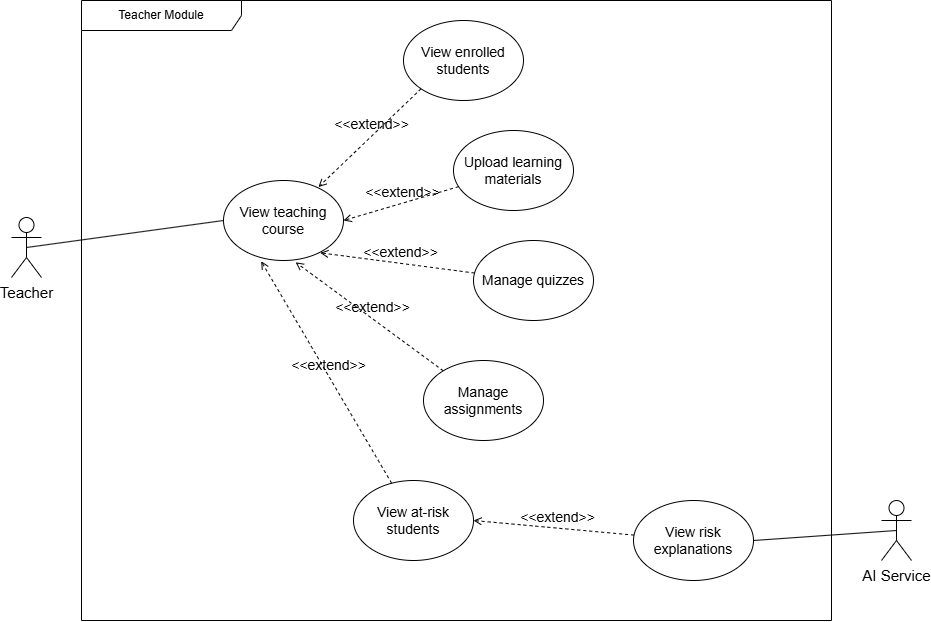
\includegraphics[width=0.8\textwidth, height=0.7\textheight, keepaspectratio]{images/usecase/teacher.png}
    \caption{Teacher Use Case Diagram}
    \label{fig:teacher-usecase}
\end{figure}

{
\renewcommand{\arraystretch}{1.1}
\setlength{\tabcolsep}{8pt}
\begin{longtable}{|>{\bfseries\raggedright\arraybackslash}p{0.205\textwidth}|>{\raggedright\arraybackslash}p{0.70\textwidth}|}
\hline
%--------------------------------------------------------------------------------
Use-case ID & UC-010 \\ \hline
%--------------------------------------------------------------------------------
Use-case name & View Teaching Course \\ \hline
%--------------------------------------------------------------------------------
Author & Thai Thien Hai Long \\ \hline
%--------------------------------------------------------------------------------
Description &
Allows the lecturer to view the Course Home Page and its overview dashboard. It serves as the central entry point for accessing learning materials, assessments, student rosters, and AI risk analytics.\\ \hline
%--------------------------------------------------------------------------------
Actor & Teacher \\ \hline
%--------------------------------------------------------------------------------
Trigger &
The teacher selects a specific course from their teaching course list on the dashboard. \\ \hline
%--------------------------------------------------------------------------------
Precondition &
1. The user is authenticated and logged in with the teacher role. \par
2. The user has been assigned to teach at least one active course by the admin. \\ \hline
%--------------------------------------------------------------------------------
Postcondition &
The course home page is displayed, presenting active course sections, announcements, and navigation links to course tools. \\ \hline
%--------------------------------------------------------------------------------
Normal Flow &
1. The teacher navigates to the ``My Courses'' section from the main navigation menu. \par
2. The system retrieves and displays the list of courses assigned to the teacher. \par
3. The teacher selects a specific course to inspect. \par
4. The system navigates to the course home page. \par
5. The system displays course sections, announcements, and existing learning materials.\\ \hline
%--------------------------------------------------------------------------------
Alternative Flow &
N/A. \\ \hline
%--------------------------------------------------------------------------------
Exception Flow &
\textbf{E1: No Assigned Courses Found} \par
1. At step 2 of the normal flow, no courses are assigned to the teacher's account. \par
2. The system displays a ``No courses'' placeholder. \par\vspace{4pt}
\textbf{E2: Course Load Failure} \par
1. At step 4 of the normal flow, the course fails to load due to a system error. \par
2. The system displays an error alert: ``Unable to load course. Please try again.'' \\ \hline
\end{longtable}
}

{
\renewcommand{\arraystretch}{1.1}
\setlength{\tabcolsep}{8pt}
\begin{longtable}{|>{\bfseries\raggedright\arraybackslash}p{0.205\textwidth}|>{\raggedright\arraybackslash}p{0.70\textwidth}|}
\hline
%--------------------------------------------------------------------------------
Use-case ID & UC-011 \\ \hline
%--------------------------------------------------------------------------------
Use-case name & View Enrolled Students \\ \hline
%--------------------------------------------------------------------------------
Author & Thai Thien Hai Long \\ \hline
%--------------------------------------------------------------------------------
Description &
Allows the teacher to view, filter, and monitor the enrolled student roster, including assigned groups and recent activity timestamps. \\ \hline
%--------------------------------------------------------------------------------
Actor & Teacher \\ \hline
%--------------------------------------------------------------------------------
Trigger &
The teacher clicks on the ``Participants'' tab from the course navigation bar. \\ \hline
%--------------------------------------------------------------------------------
Precondition &
1. The user is authenticated and logged in with the Teacher role.\par
2. The user has accessed the target course home page. \\ \hline
%--------------------------------------------------------------------------------
Postcondition &
The enrolled student roster is displayed, including student IDs, full names, assigned groups, and last access timestamps. \\ \hline
%--------------------------------------------------------------------------------
Normal Flow &
1. From the course home page, the teacher selects the ``Participants'' tab.\par
2. The system queries the database for all enrolled users associated with the course.\par
3. The system displays the participant table containing student names, ID numbers, email addresses, assigned groups, roles, and last access timestamps. \\ \hline
%--------------------------------------------------------------------------------
Alternative Flow &
\textbf{A1: Filter or Search Students}\par
1. At step 3 of the normal flow, the teacher enters a search keyword or selects a class group filter. \par
2. The system filters and displays the matching subset of enrolled students. \\ \hline
%--------------------------------------------------------------------------------
Exception Flow &
\textbf{E1: No Students Enrolled}\par
1. At step 2 of the normal flow, no student records are linked to the course.\par
2. The system displays an empty-state message: ``No participants found in this course.''\par\vspace{4pt}
\textbf{E2: Participant Data Load Failure}\par
1. At step 2 of the normal flow, the participant list fails to load due to a database connection error.\par
2. The system displays an error alert: ``Unable to retrieve participant list. Please refresh the page.'' \\ \hline
%--------------------------------------------------------------------------------
\end{longtable}
}

{
\renewcommand{\arraystretch}{1.1}
\setlength{\tabcolsep}{8pt}
\begin{longtable}{|>{\bfseries\raggedright\arraybackslash}p{0.21\textwidth}|>{\raggedright\arraybackslash}p{0.70\textwidth}|}
\hline
%--------------------------------------------------------------------------------
Use-case ID & UC-012 \\ \hline
%--------------------------------------------------------------------------------
Use-case name & Upload Learning Materials \\ \hline
%--------------------------------------------------------------------------------
Author & Thai Thien Hai Long \\ \hline
%--------------------------------------------------------------------------------
Description &
Allows the teacher to add learning resources (e.g., lecture slides, documents, syllabus, or links) to specific course sections for enrolled students to access. \\ \hline
%--------------------------------------------------------------------------------
Actor & Teacher \\ \hline
%--------------------------------------------------------------------------------
Trigger &
The teacher enables edit mode and selects ``Add an activity or resource'' within a course section. \\ \hline
%--------------------------------------------------------------------------------
Precondition &
1. The user is authenticated and logged in with the Teacher role. \par
2. The user has accessed the target course home page. \\ \hline
%--------------------------------------------------------------------------------
Postcondition &
The uploaded learning material is saved and displayed within the selected course section. \\ \hline
%--------------------------------------------------------------------------------
Normal Flow &
1. From the course home page, the teacher turns on ``Edit mode''. \par
2. In the target section, the teacher clicks ``Add an activity or resource'' and selects ``File'' (or ``Folder''). \par
3. The system displays the resource setup form. \par
4. The teacher inputs the resource name, description, and uploads the file attachment. \par
5. The teacher clicks ``Save and return to course''. \par
6. The system validates the file, stores it, and displays the new resource link in the course section. \\ \hline
%--------------------------------------------------------------------------------
Alternative Flow &
\textbf{A1: Upload via Drag-and-Drop} \par
1. At step 2 of the normal flow, the teacher directly drags and drops a file from the local file explorer into the desired section on the course page. \par
2. The system automatically uploads the file and creates a resource entry using the filename. \par\vspace{4pt}
\textbf{A2: Add External URL Resource} \par
1. At step 2 of the normal flow, the teacher selects ``URL'' instead of ``File''. \par
2. The teacher enters the resource title and external web address. \par
3. The flow proceeds to step 5. \\ \hline
%--------------------------------------------------------------------------------
Exception Flow &
\textbf{E1: File Size Exceeds Limit} \par
1. At step 5 of the normal flow, the uploaded file exceeds the course upload size limit. \par
2. The system rejects the file and displays an alert: ``The file is too large to be uploaded.'' \par
3. The flow returns to step 4 for file re-selection. \par\vspace{4pt}
\textbf{E2: Unsupported File Format} \par
1. At step 5 of the normal flow, the file format is restricted by system policy. \par
2. The system displays an error: ``This file type is not allowed.'' \par
3. The flow returns to step 4. \\ \hline
\end{longtable}
}

{
\renewcommand{\arraystretch}{1.1}
\setlength{\tabcolsep}{8pt}
\begin{longtable}{|>{\bfseries\raggedright\arraybackslash}p{0.21\textwidth}|>{\raggedright\arraybackslash}p{0.70\textwidth}|}
\hline
%--------------------------------------------------------------------------------
Use-case ID & UC-013 \\ \hline
%--------------------------------------------------------------------------------
Use-case name & Manage Quizzes \\ \hline
%--------------------------------------------------------------------------------
Author & Thai Thien Hai Long \\ \hline
%--------------------------------------------------------------------------------
Description &
Allows the teacher to create, configure, update, or remove online quiz assessments and define question sets and grading rules for the course. \\ \hline
%--------------------------------------------------------------------------------
Actor & Teacher \\ \hline
%--------------------------------------------------------------------------------
Trigger &
The teacher enables edit mode and selects ``Add an activity or resource'' > ``Quiz'' within a course section. \\ \hline
%--------------------------------------------------------------------------------
Precondition &
1. The user is authenticated and logged in with the Teacher role. \par
2. The user has accessed the target course home page. \\ \hline
%--------------------------------------------------------------------------------
Postcondition &
The quiz activity and its configured question items are saved and published in the designated course section. \\ \hline
%--------------------------------------------------------------------------------
Normal Flow &
1. From the course home page, the teacher turns on ``Edit mode''. \par
2. In the target section, the teacher clicks ``Add an activity or resource'' and selects ``Quiz''. \par
3. The system displays the quiz settings page (timing, grade boundaries, attempt limits). \par
4. The teacher configures the quiz parameters and clicks ``Save and display''. \par
5. The system opens the quiz question management interface. \par
6. The teacher adds questions from the question bank or creates new questions with point values. \par
7. The teacher saves the assessment. \par
8. The system updates the quiz structure and makes it accessible in the course section. \\ \hline
%--------------------------------------------------------------------------------
Alternative Flow &
\textbf{A1: Edit Existing Quiz} \par
1. At step 2 of the normal flow, the teacher clicks the action menu of an existing quiz and selects ``Edit settings''. \par
2. The system loads existing configurations and questions. \par
3. The teacher updates parameters or modifies questions. \par
4. The flow proceeds to step 7. \par\vspace{4pt}
\textbf{A2: Delete Quiz} \par
1. At step 2 of the normal flow, the teacher selects ``Delete'' on an existing quiz. \par
2. The system requests confirmation. \par
3. The teacher confirms deletion, and the system removes the quiz activity from the course. \\ \hline
%--------------------------------------------------------------------------------
Exception Flow &
\textbf{E1: Invalid Time Window} \par
1. At step 4 of the normal flow, the quiz close time is configured before the open time. \par
2. The system displays a validation error: ``The closing time cannot be earlier than the opening time.'' \par
3. The teacher adjusts the timestamps. \par\vspace{4pt}
\textbf{E2: Empty Question Set} \par
1. At step 7 of the normal flow, the teacher attempts to publish a quiz without adding any questions. \par
2. The system displays a warning notice: ``No questions have been added yet.'' \\ \hline
\end{longtable}
}

{
\renewcommand{\arraystretch}{1.1}
\setlength{\tabcolsep}{8pt}
\begin{longtable}{|>{\bfseries\raggedright\arraybackslash}p{0.21\textwidth}|>{\raggedright\arraybackslash}p{0.70\textwidth}|}
\hline
%--------------------------------------------------------------------------------
Use-case ID & UC-014 \\ \hline
%--------------------------------------------------------------------------------
Use-case name & Manage Assignments \\ \hline
%--------------------------------------------------------------------------------
Author & Thai Thien Hai Long \\ \hline
%--------------------------------------------------------------------------------
Description &
Allows the teacher to create, configure, update, or remove student assignment dropboxes, specifying submission formats, deadlines, and grading criteria. \\ \hline
%--------------------------------------------------------------------------------
Actor & Teacher \\ \hline
%--------------------------------------------------------------------------------
Trigger &
The teacher enables edit mode and selects ``Add an activity or resource'' > ``Assignment'' within a course section. \\ \hline
%--------------------------------------------------------------------------------
Precondition &
1. The user is authenticated and logged in with the Teacher role. \par
2. The user has accessed the target course home page. \\ \hline
%--------------------------------------------------------------------------------
Postcondition &
The assignment entry is created or updated, providing an active submission portal for enrolled students. \\ \hline
%--------------------------------------------------------------------------------
Normal Flow &
1. From the course home page, the teacher turns on ``Edit mode''. \par
2. In the target section, the teacher clicks ``Add an activity or resource'' and selects ``Assignment''. \par
3. The system displays the assignment configuration form. \par
4. The teacher specifies assignment title, description instructions, and optional prompt attachments. \par
5. The teacher configures availability dates (allow submissions from, due date, cutoff date) and file submission limits. \par
6. The teacher clicks ``Save and return to course''. \par
7. The system validates the submission parameters and publishes the assignment item. \\ \hline
%--------------------------------------------------------------------------------
Alternative Flow &
\textbf{A1: Edit Existing Assignment} \par
1. At step 2 of the normal flow, the teacher clicks the action menu of an existing assignment and selects ``Edit settings''. \par
2. The system populates the form with existing assignment configurations. \par
3. The teacher updates instructions or extends deadlines. \par
4. The flow proceeds to step 6. \par\vspace{4pt}
\textbf{A2: Delete Assignment} \par
1. At step 2 of the normal flow, the teacher selects ``Delete'' on an existing assignment. \par
2. The system prompts a confirmation dialog. \par
3. The teacher confirms deletion, and the system removes the assignment. \\ \hline
%--------------------------------------------------------------------------------
Exception Flow &
\textbf{E1: Invalid Due Date} \par
1. At step 6 of the normal flow, the specified due date precedes the allowable submission start date. \par
2. The system halts submission and displays an error: ``Due date must be after the allow submissions from date.'' \par
3. The flow returns to step 5. \par\vspace{4pt}
\textbf{E2: File Size Exceeds Limit} \par
1. At step 4 of the normal flow, the attached assignment prompt file exceeds maximum upload size. \par
2. The system rejects the file and displays an error alert: ``The uploaded instruction file exceeds size limits.'' \\ \hline
\end{longtable}
}

{
\renewcommand{\arraystretch}{1.1}
\setlength{\tabcolsep}{8pt}
\begin{longtable}{|>{\bfseries\raggedright\arraybackslash}p{0.21\textwidth}|>{\raggedright\arraybackslash}p{0.70\textwidth}|}
\hline
%--------------------------------------------------------------------------------
Use-case ID & UC-015 \\ \hline
%--------------------------------------------------------------------------------
Use-case name & View At-Risk Students and Risk Explanations \\ \hline
%--------------------------------------------------------------------------------
Author & Thai Thien Hai Long \\ \hline
%--------------------------------------------------------------------------------
Description &
Allows the teacher to review an AI-analyzed roster of enrolled students at academic risk within a specific course, inspect feature-based explanations (e.g., inactivity duration, assignment delays, or quiz drop-offs), and trigger personalized outreach interventions. \\ \hline
%--------------------------------------------------------------------------------
Actor & Teacher, AI Service (Secondary) \\ \hline
%--------------------------------------------------------------------------------
Trigger &
The teacher navigates to the ``Analytics / At-Risk Students'' section from the course management dashboard. \\ \hline
%--------------------------------------------------------------------------------
Precondition &
1. The user is authenticated and logged in with the Teacher role. \par
2. The user has accessed a course they are actively assigned to teach. \par
3. The background feature extraction and AI prediction pipeline has processed current student activity and grade logs. \\ \hline
%--------------------------------------------------------------------------------
Postcondition &
The teacher reviews categorized student risk profiles and explanations, and optional intervention actions (e.g., outreach email logs) are recorded. \\ \hline
%--------------------------------------------------------------------------------
Normal Flow &
1. From the course home page, the teacher navigates to the ``At-Risk Students'' analytics overview. \par
2. The system queries the AI service and displays the student roster categorized into risk levels (\textit{High Risk}, \textit{Medium Risk}, \textit{Safe}). \par
3. The teacher filters or sorts the roster by risk severity or student identifier. \par
4. The teacher selects a flagged student to view detailed risk indicators. \par
5. The system requests the explanation payload from the AI service. \par
6. The AI service computes/retrieves feature attributions and returns plain-language pedagogical reasons (e.g., prolonged inactivity, negative quiz score slopes, missing submissions). \par
7. The system renders the student risk profile along with the primary contributing factors and impact weights. \par
8. The teacher reviews the assessment and closes or acknowledges the report. \\ \hline
%--------------------------------------------------------------------------------
Alternative Flow &
\textbf{A1: Generate AI Intervention Outreach} \par
1. At step 7 of the normal flow, the teacher clicks ``Draft Personalized Outreach''. \par
2. The system prompts the generative AI service with the student's contributing risk factors to draft an empathetic email. \par
3. The teacher reviews, edits, and sends the drafted communication. \par
4. The system logs the intervention status and returns to step 3. \par\vspace{4pt}
\textbf{A2: Filter by Safe or Moderate Thresholds} \par
1. At step 3 of the normal flow, the teacher selects a filter to inspect stable or low-risk students. \par
2. The system updates the roster view to show students whose performance indicators meet course baselines. \\ \hline
%--------------------------------------------------------------------------------
Exception Flow &
\textbf{E1: Insufficient Activity Data for Evaluation} \par
1. At step 2 of the normal flow, the course has insufficient student interaction logs or submission records to compute reliable risk predictions. \par
2. The system displays an informational status banner: ``Insufficient activity data available to generate early warning predictions.'' \par
3. The flow terminates without rendering risk tiers. \par\vspace{4pt}
\textbf{E2: AI Service / Analytics Endpoint Unavailable} \par
1. At step 2 or step 5 of the normal flow, the connection to the AI analytics microservice times out or returns an error. \par
2. The system displays a notification alert: ``Unable to retrieve predictive analytics. Please try again later.'' \par
3. The system falls back to displaying raw gradebook summaries without AI risk classifications. \\ \hline
\end{longtable}
}